% Options for packages loaded elsewhere
\PassOptionsToPackage{unicode}{hyperref}
\PassOptionsToPackage{hyphens}{url}
%
\documentclass[
  ignorenonframetext,
]{beamer}
\usepackage{pgfpages}
\setbeamertemplate{caption}[numbered]
\setbeamertemplate{caption label separator}{: }
\setbeamercolor{caption name}{fg=normal text.fg}
\beamertemplatenavigationsymbolsempty
% Prevent slide breaks in the middle of a paragraph
\widowpenalties 1 10000
\raggedbottom
\setbeamertemplate{part page}{
  \centering
  \begin{beamercolorbox}[sep=16pt,center]{part title}
    \usebeamerfont{part title}\insertpart\par
  \end{beamercolorbox}
}
\setbeamertemplate{section page}{
  \centering
  \begin{beamercolorbox}[sep=12pt,center]{part title}
    \usebeamerfont{section title}\insertsection\par
  \end{beamercolorbox}
}
\setbeamertemplate{subsection page}{
  \centering
  \begin{beamercolorbox}[sep=8pt,center]{part title}
    \usebeamerfont{subsection title}\insertsubsection\par
  \end{beamercolorbox}
}
\AtBeginPart{
  \frame{\partpage}
}
\AtBeginSection{
  \ifbibliography
  \else
    \frame{\sectionpage}
  \fi
}
\AtBeginSubsection{
  \frame{\subsectionpage}
}
\usepackage{amsmath,amssymb}
\usepackage{iftex}
\ifPDFTeX
  \usepackage[T1]{fontenc}
  \usepackage[utf8]{inputenc}
  \usepackage{textcomp} % provide euro and other symbols
\else % if luatex or xetex
  \usepackage{unicode-math} % this also loads fontspec
  \defaultfontfeatures{Scale=MatchLowercase}
  \defaultfontfeatures[\rmfamily]{Ligatures=TeX,Scale=1}
\fi
\usepackage{lmodern}
\ifPDFTeX\else
  % xetex/luatex font selection
\fi
% Use upquote if available, for straight quotes in verbatim environments
\IfFileExists{upquote.sty}{\usepackage{upquote}}{}
\IfFileExists{microtype.sty}{% use microtype if available
  \usepackage[]{microtype}
  \UseMicrotypeSet[protrusion]{basicmath} % disable protrusion for tt fonts
}{}
\makeatletter
\@ifundefined{KOMAClassName}{% if non-KOMA class
  \IfFileExists{parskip.sty}{%
    \usepackage{parskip}
  }{% else
    \setlength{\parindent}{0pt}
    \setlength{\parskip}{6pt plus 2pt minus 1pt}}
}{% if KOMA class
  \KOMAoptions{parskip=half}}
\makeatother
\usepackage{xcolor}
\newif\ifbibliography
\usepackage{color}
\usepackage{fancyvrb}
\newcommand{\VerbBar}{|}
\newcommand{\VERB}{\Verb[commandchars=\\\{\}]}
\DefineVerbatimEnvironment{Highlighting}{Verbatim}{commandchars=\\\{\}}
% Add ',fontsize=\small' for more characters per line
\usepackage{framed}
\definecolor{shadecolor}{RGB}{248,248,248}
\newenvironment{Shaded}{\begin{snugshade}}{\end{snugshade}}
\newcommand{\AlertTok}[1]{\textcolor[rgb]{0.94,0.16,0.16}{#1}}
\newcommand{\AnnotationTok}[1]{\textcolor[rgb]{0.56,0.35,0.01}{\textbf{\textit{#1}}}}
\newcommand{\AttributeTok}[1]{\textcolor[rgb]{0.13,0.29,0.53}{#1}}
\newcommand{\BaseNTok}[1]{\textcolor[rgb]{0.00,0.00,0.81}{#1}}
\newcommand{\BuiltInTok}[1]{#1}
\newcommand{\CharTok}[1]{\textcolor[rgb]{0.31,0.60,0.02}{#1}}
\newcommand{\CommentTok}[1]{\textcolor[rgb]{0.56,0.35,0.01}{\textit{#1}}}
\newcommand{\CommentVarTok}[1]{\textcolor[rgb]{0.56,0.35,0.01}{\textbf{\textit{#1}}}}
\newcommand{\ConstantTok}[1]{\textcolor[rgb]{0.56,0.35,0.01}{#1}}
\newcommand{\ControlFlowTok}[1]{\textcolor[rgb]{0.13,0.29,0.53}{\textbf{#1}}}
\newcommand{\DataTypeTok}[1]{\textcolor[rgb]{0.13,0.29,0.53}{#1}}
\newcommand{\DecValTok}[1]{\textcolor[rgb]{0.00,0.00,0.81}{#1}}
\newcommand{\DocumentationTok}[1]{\textcolor[rgb]{0.56,0.35,0.01}{\textbf{\textit{#1}}}}
\newcommand{\ErrorTok}[1]{\textcolor[rgb]{0.64,0.00,0.00}{\textbf{#1}}}
\newcommand{\ExtensionTok}[1]{#1}
\newcommand{\FloatTok}[1]{\textcolor[rgb]{0.00,0.00,0.81}{#1}}
\newcommand{\FunctionTok}[1]{\textcolor[rgb]{0.13,0.29,0.53}{\textbf{#1}}}
\newcommand{\ImportTok}[1]{#1}
\newcommand{\InformationTok}[1]{\textcolor[rgb]{0.56,0.35,0.01}{\textbf{\textit{#1}}}}
\newcommand{\KeywordTok}[1]{\textcolor[rgb]{0.13,0.29,0.53}{\textbf{#1}}}
\newcommand{\NormalTok}[1]{#1}
\newcommand{\OperatorTok}[1]{\textcolor[rgb]{0.81,0.36,0.00}{\textbf{#1}}}
\newcommand{\OtherTok}[1]{\textcolor[rgb]{0.56,0.35,0.01}{#1}}
\newcommand{\PreprocessorTok}[1]{\textcolor[rgb]{0.56,0.35,0.01}{\textit{#1}}}
\newcommand{\RegionMarkerTok}[1]{#1}
\newcommand{\SpecialCharTok}[1]{\textcolor[rgb]{0.81,0.36,0.00}{\textbf{#1}}}
\newcommand{\SpecialStringTok}[1]{\textcolor[rgb]{0.31,0.60,0.02}{#1}}
\newcommand{\StringTok}[1]{\textcolor[rgb]{0.31,0.60,0.02}{#1}}
\newcommand{\VariableTok}[1]{\textcolor[rgb]{0.00,0.00,0.00}{#1}}
\newcommand{\VerbatimStringTok}[1]{\textcolor[rgb]{0.31,0.60,0.02}{#1}}
\newcommand{\WarningTok}[1]{\textcolor[rgb]{0.56,0.35,0.01}{\textbf{\textit{#1}}}}
\usepackage{graphicx}
\makeatletter
\def\maxwidth{\ifdim\Gin@nat@width>\linewidth\linewidth\else\Gin@nat@width\fi}
\def\maxheight{\ifdim\Gin@nat@height>\textheight\textheight\else\Gin@nat@height\fi}
\makeatother
% Scale images if necessary, so that they will not overflow the page
% margins by default, and it is still possible to overwrite the defaults
% using explicit options in \includegraphics[width, height, ...]{}
\setkeys{Gin}{width=\maxwidth,height=\maxheight,keepaspectratio}
% Set default figure placement to htbp
\makeatletter
\def\fps@figure{htbp}
\makeatother
\setlength{\emergencystretch}{3em} % prevent overfull lines
\providecommand{\tightlist}{%
  \setlength{\itemsep}{0pt}\setlength{\parskip}{0pt}}
\setcounter{secnumdepth}{-\maxdimen} % remove section numbering
\ifLuaTeX
  \usepackage{selnolig}  % disable illegal ligatures
\fi
\IfFileExists{bookmark.sty}{\usepackage{bookmark}}{\usepackage{hyperref}}
\IfFileExists{xurl.sty}{\usepackage{xurl}}{} % add URL line breaks if available
\urlstyle{same}
\hypersetup{
  pdftitle={Giorno 1 Geostatistica - corso base},
  pdfauthor={Francesco Pirotti},
  hidelinks,
  pdfcreator={LaTeX via pandoc}}

\title{Giorno 1 Geostatistica - corso base}
\author{Francesco Pirotti}
\date{2024-05-27}

\begin{document}
\frame{\titlepage}

\begin{frame}{Cosa impareremo}
\protect\hypertarget{cosa-impareremo}{}
\begin{itemize}
\tightlist
\item
  struttura di R (base e pacchetti), potenzialità
\item
  RStudio: come funziona (panoramica)
\item
  Documentazione, esempi, snippets per imparare
\item
  assegnazione ed utilizzo variabili
\item
  principali strutture dati: oggetti e funzioni in R
\item
  leggere e scrivere dati tabellari e complessi
\end{itemize}
\end{frame}

\begin{frame}{Introduzione}
\protect\hypertarget{introduzione}{}
\begin{itemize}
\tightlist
\item
  struttura di R - percorso di installazione
\end{itemize}

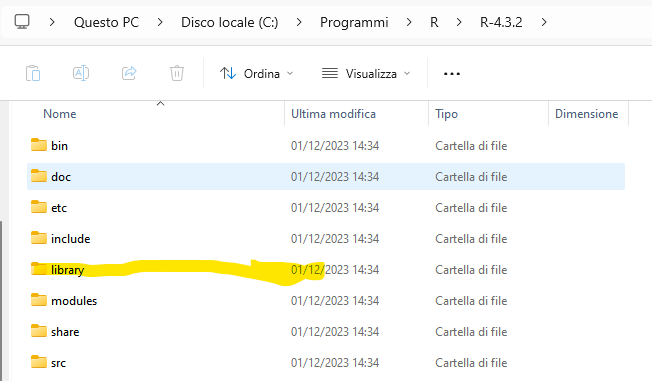
\includegraphics{images/clipboard-431216307.png}
\end{frame}

\begin{frame}{RStudio}
\protect\hypertarget{rstudio}{}
\begin{itemize}
\tightlist
\item
  versione desktop/server
\item
  vantaggi interfaccia:

  \begin{itemize}
  \tightlist
  \item
    console/terminale/background
  \item
    progetti/packages/help
  \item
    Environment/History/Connection/Tutorial
  \end{itemize}
\end{itemize}

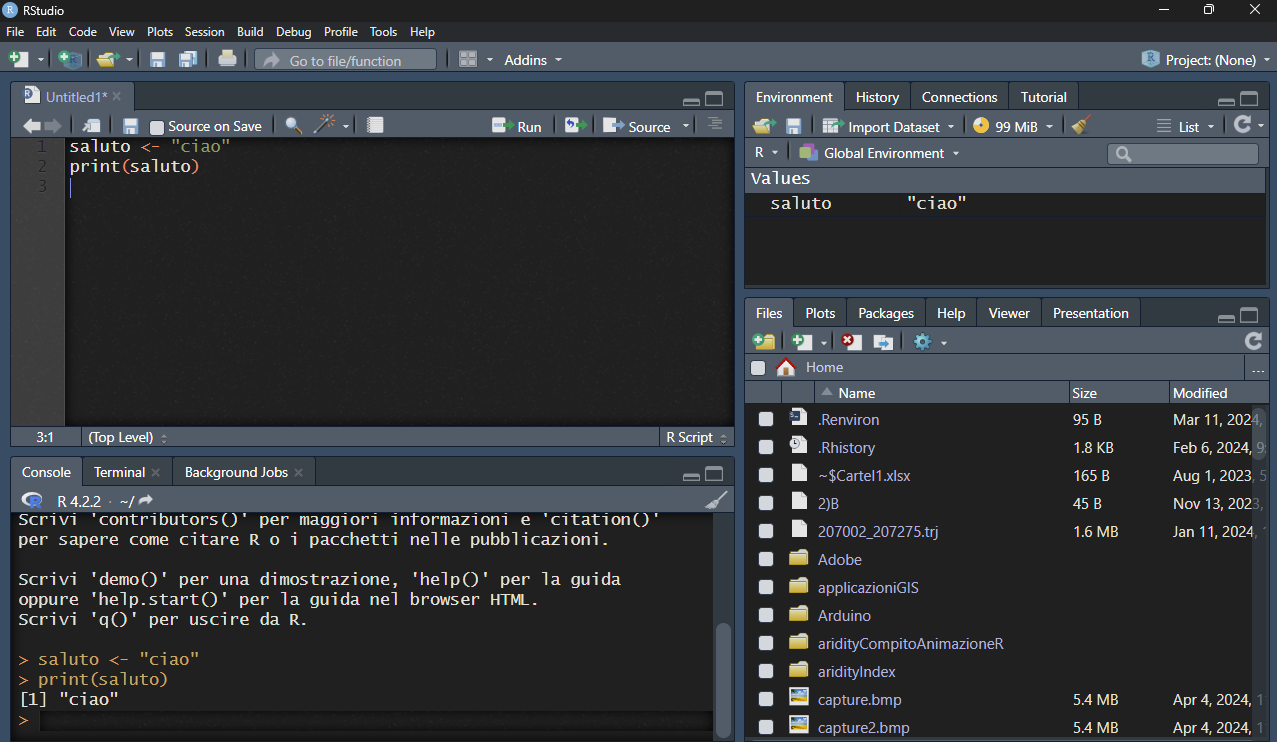
\includegraphics[width=10in,height=\textheight]{images/clipboard-3935879104.png}
\end{frame}

\begin{frame}[fragile]{Immissione dei comandi}
\protect\hypertarget{immissione-dei-comandi}{}
R è un programma basato su righe di comando.

L'utente immette i comandi al prompt ( \textgreater{} ) e ciascun
comando viene eseguito uno alla volta andando a capo.

Le righe di comando solitamente vengono salvate in un file ``script''
con estensione ``R'' (.R) e vengono eseguite una alla volta mediante
``invio'' o con selezione multipla e ``invio''.

Con RStudio è possibile eseguire l'intero file, fermandosi eventualmente
in punti specifici ``breakpoints'' (lo vedremo durante il corso)

\begin{block}{Esercizio:}
\protect\hypertarget{esercizio}{}
esegui comando della figura alla \protect\hyperlink{}{slide precedente}.

\begin{Shaded}
\begin{Highlighting}[]
\NormalTok{saluto }\OtherTok{\textless{}{-}} \StringTok{"ciao"}
\FunctionTok{print}\NormalTok{(saluto)}
\end{Highlighting}
\end{Shaded}

\begin{verbatim}
## [1] "ciao"
\end{verbatim}
\end{block}
\end{frame}

\begin{frame}[fragile]{Documentazione, esempi, snippets per imparare}
\protect\hypertarget{documentazione-esempi-snippets-per-imparare}{}
Ogni singola funzione ha ampia documentazione con molti esempi.
Chiamando una funzione dopo uno o due punti interrogativi richiama la
documentazione. Quasi sempre gli esempi sono eseguibili facendo
copia/incolla

\begin{block}{Esercizio:}
\protect\hypertarget{esercizio-1}{}
esegui il primo esempio dalla documentazione della funzione \emph{print}

\begin{Shaded}
\begin{Highlighting}[]
\NormalTok{?print}
\NormalTok{??print}
\end{Highlighting}
\end{Shaded}
\end{block}
\end{frame}

\begin{frame}[fragile]{Variabili e funzioni (parte 1)}
\protect\hypertarget{variabili-e-funzioni-parte-1}{}
Qui vediamo una variabile ed una funzione.

\textbf{NB1} - la variabile ``saluto'' è nel environment
(``ambito/ambiente/campo'') \emph{globale*}. La funzione ``print'' è nel
cmapo del package ``base'' - tieni premuto il tasto CTRL e seleziona il
nome della funzione - vedi cosa succede.

\textbf{NB2} - operatore di assegnazione \texttt{\textless{}-} (o
\texttt{\textless{}\textless{}-} nel caso si voglia forzare
l'assegnazione ad una variabile \emph{globale*})

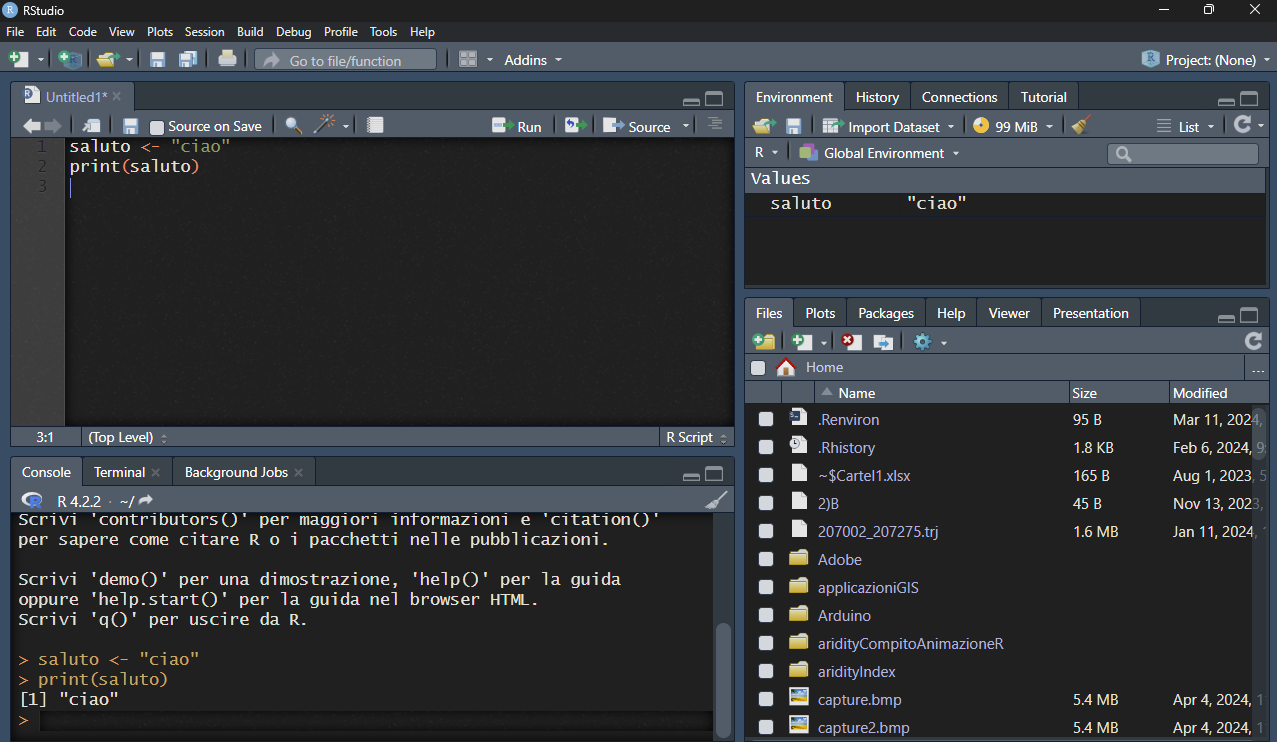
\includegraphics[width=10in,height=\textheight]{images/clipboard-3935879104.png}
\end{frame}

\begin{frame}[fragile]{Variabili e funzioni (parte 1) - Scope}
\protect\hypertarget{variabili-e-funzioni-parte-1---scope}{}
*Le variabili create al di fuori di funzioni sono note come variabili
\textbf{\emph{globali};} possono essere utilizzate sia all'interno delle
funzioni che all'esterno.

Sotto andiamo a creare una nostra funzione ``salutami'' che esegue il
saluto. Provate a modificare l'operatore di assegnazione da
\texttt{\textless{}\textless{}-} a \texttt{\textless{}\textless{}-} e
rieseguire!!

\begin{Shaded}
\begin{Highlighting}[]
\NormalTok{salutami }\OtherTok{\textless{}{-}} \ControlFlowTok{function}\NormalTok{()\{}
\NormalTok{  saluto }\OtherTok{\textless{}{-}} \StringTok{"ciao ARPA!!!"}
  \FunctionTok{print}\NormalTok{(saluto)}
\NormalTok{\}}

\FunctionTok{print}\NormalTok{(saluto)}
\end{Highlighting}
\end{Shaded}

\begin{verbatim}
## [1] "ciao"
\end{verbatim}

\begin{Shaded}
\begin{Highlighting}[]
\FunctionTok{salutami}\NormalTok{()}
\end{Highlighting}
\end{Shaded}

\begin{verbatim}
## [1] "ciao ARPA!!!"
\end{verbatim}

\begin{Shaded}
\begin{Highlighting}[]
\FunctionTok{print}\NormalTok{(saluto)}
\end{Highlighting}
\end{Shaded}

\begin{verbatim}
## [1] "ciao"
\end{verbatim}
\end{frame}

\begin{frame}[fragile]{Strutture dati in R}
\protect\hypertarget{strutture-dati-in-r}{}
NB ogni elemento in R è considerato (ed è) un VETTORE. Le funzioni di R
considerano ogni variabile un vettore. Cosa significa? Che le funzioni
elaborano tutti gli elementi di un vettore ``by default'' e che ogni
elemento è indicabile con un numero iniziando da 1 (non da 0 come
solitamente succede in altri linguaggi).

\begin{itemize}
\tightlist
\item
  vector
\item
  character
\item
  integer
\item
  numeric
\end{itemize}

\begin{Shaded}
\begin{Highlighting}[]
\NormalTok{miaVar }\OtherTok{\textless{}{-}} \ConstantTok{FALSE}
\FunctionTok{class}\NormalTok{(miaVar)}
\NormalTok{miaVar[[}\DecValTok{1}\NormalTok{]]}
\NormalTok{miaVar[[}\DecValTok{2}\NormalTok{]]}
\end{Highlighting}
\end{Shaded}
\end{frame}

\begin{frame}[fragile]{Strutture dati- vettori}
\protect\hypertarget{strutture-dati--vettori}{}
\begin{block}{Esercizio:}
\protect\hypertarget{esercizio-2}{}
perchè succede quello che vedete sotto?

\begin{Shaded}
\begin{Highlighting}[]
\NormalTok{miaVar }\OtherTok{\textless{}{-}} \FunctionTok{c}\NormalTok{(}\DecValTok{1}\NormalTok{,}\DecValTok{4}\NormalTok{,}\DecValTok{6}\NormalTok{,}\DecValTok{8}\NormalTok{)}
\FunctionTok{class}\NormalTok{(miaVar)}
\end{Highlighting}
\end{Shaded}

\begin{verbatim}
## [1] "numeric"
\end{verbatim}

\begin{Shaded}
\begin{Highlighting}[]
\NormalTok{miaVar[[}\DecValTok{1}\NormalTok{]]}
\end{Highlighting}
\end{Shaded}

\begin{verbatim}
## [1] 1
\end{verbatim}

\begin{Shaded}
\begin{Highlighting}[]
\NormalTok{miaVar[[}\DecValTok{2}\NormalTok{]]}
\end{Highlighting}
\end{Shaded}

\begin{verbatim}
## [1] 4
\end{verbatim}

\begin{Shaded}
\begin{Highlighting}[]
\NormalTok{miaVar[[}\DecValTok{2}\NormalTok{]] }\OtherTok{\textless{}{-}} \StringTok{"evviva"}
\FunctionTok{class}\NormalTok{(miaVar)}
\end{Highlighting}
\end{Shaded}

\begin{verbatim}
## [1] "character"
\end{verbatim}

\begin{Shaded}
\begin{Highlighting}[]
\FunctionTok{print}\NormalTok{(miaVar)}
\end{Highlighting}
\end{Shaded}

\begin{verbatim}
## [1] "1"      "evviva" "6"      "8"
\end{verbatim}
\end{block}
\end{frame}

\begin{frame}[fragile]{Strutture dati- matrix}
\protect\hypertarget{strutture-dati--matrix}{}
Matrix è un oggetto con struttura di matrice ovvero bidimensionale
(righe × colonne); pensate a un gruppo di vettori impilati o affiancati.

Si accede e si assegnano i valori con {[}r,c{]} dove r e ci sono gli
indici di riga e colonna. Si può lasciare vuoto un indice per accedere
alla riga/colonna

\begin{Shaded}
\begin{Highlighting}[]
\NormalTok{mat }\OtherTok{\textless{}{-}} \FunctionTok{matrix}\NormalTok{(}\FunctionTok{c}\NormalTok{(}\DecValTok{1}\NormalTok{, }\DecValTok{2}\NormalTok{, }\DecValTok{3}\NormalTok{, }\DecValTok{4}\NormalTok{), }\AttributeTok{nrow =} \DecValTok{2}\NormalTok{, }\AttributeTok{ncol =} \DecValTok{2}\NormalTok{)}
\NormalTok{mat[[}\DecValTok{2}\NormalTok{]]}
\end{Highlighting}
\end{Shaded}

\begin{verbatim}
## [1] 2
\end{verbatim}

\begin{Shaded}
\begin{Highlighting}[]
\NormalTok{mat[}\DecValTok{1}\NormalTok{,}\DecValTok{2}\NormalTok{]}
\end{Highlighting}
\end{Shaded}

\begin{verbatim}
## [1] 3
\end{verbatim}

\begin{Shaded}
\begin{Highlighting}[]
\NormalTok{mat[}\DecValTok{1}\NormalTok{,]}
\end{Highlighting}
\end{Shaded}

\begin{verbatim}
## [1] 1 3
\end{verbatim}

\begin{Shaded}
\begin{Highlighting}[]
\NormalTok{mat[}\DecValTok{1}\NormalTok{,}\DecValTok{2}\NormalTok{] }\OtherTok{\textless{}{-}} \DecValTok{100}
\end{Highlighting}
\end{Shaded}
\end{frame}

\begin{frame}[fragile]{Strutture dati- array}
\protect\hypertarget{strutture-dati--array}{}
Un array è una matrice multidimensionale.

r=rows, c=columns, m=matrice\ldots. etc\ldots{}

\begin{block}{Esercizio:}
\protect\hypertarget{esercizio-3}{}
Vedi sotto come creare un array a 3 dimensioni. Nota che duplica 9
valori 2 volte. Prova a dare 8 valori invece che nove. Prova a dare 3
valori. Cosa succede.

\begin{Shaded}
\begin{Highlighting}[]
\CommentTok{\# 2 vettori di valori }
\NormalTok{valori1 }\OtherTok{\textless{}{-}} \FunctionTok{c}\NormalTok{(}\DecValTok{5}\NormalTok{, }\DecValTok{9}\NormalTok{, }\DecValTok{3}\NormalTok{) }
\NormalTok{valori2 }\OtherTok{\textless{}{-}} \FunctionTok{c}\NormalTok{(}\DecValTok{10}\NormalTok{, }\DecValTok{11}\NormalTok{, }\DecValTok{12}\NormalTok{, }\DecValTok{13}\NormalTok{, }\DecValTok{14}\NormalTok{, }\DecValTok{15}\NormalTok{) }
\NormalTok{column.names }\OtherTok{\textless{}{-}} \FunctionTok{c}\NormalTok{(}\StringTok{"C1"}\NormalTok{, }\StringTok{"C2"}\NormalTok{, }\StringTok{"C3"}\NormalTok{) }
\NormalTok{row.names }\OtherTok{\textless{}{-}} \FunctionTok{c}\NormalTok{(}\StringTok{"R1"}\NormalTok{, }\StringTok{"R2"}\NormalTok{, }\StringTok{"R3"}\NormalTok{) }
\NormalTok{matrix.names }\OtherTok{\textless{}{-}} \FunctionTok{c}\NormalTok{(}\StringTok{"Matrix1"}\NormalTok{, }\StringTok{"Matrix2"}\NormalTok{) }
  
\CommentTok{\# Take these vectors as input to the array. }
\NormalTok{result }\OtherTok{\textless{}{-}} \FunctionTok{array}\NormalTok{(}\FunctionTok{c}\NormalTok{(valori1, valori2), }\AttributeTok{dim =} \FunctionTok{c}\NormalTok{(}\DecValTok{3}\NormalTok{, }\DecValTok{3}\NormalTok{, }\DecValTok{2}\NormalTok{), }
                  \AttributeTok{dimnames =} \FunctionTok{list}\NormalTok{(row.names, }
\NormalTok{                                  column.names, }
\NormalTok{                                  matrix.names)) }
\FunctionTok{print}\NormalTok{(result) }
\end{Highlighting}
\end{Shaded}

\begin{verbatim}
## , , Matrix1
## 
##    C1 C2 C3
## R1  5 10 13
## R2  9 11 14
## R3  3 12 15
## 
## , , Matrix2
## 
##    C1 C2 C3
## R1  5 10 13
## R2  9 11 14
## R3  3 12 15
\end{verbatim}
\end{block}
\end{frame}

\begin{frame}[fragile]{Strutture dati- list}
\protect\hypertarget{strutture-dati--list}{}
Le strutture vector/matrix/array, possono contenere solo una tipologia
base (numeric, integer, character, logical\ldots). Ma la struttura LIST
no!

La struttura \emph{list} è un set di dati eterogenei; opzionalmente, è
possibile assegnare dei nomi a ciascun elemento nel set.

\begin{Shaded}
\begin{Highlighting}[]
\NormalTok{lista }\OtherTok{\textless{}{-}} \FunctionTok{list}\NormalTok{(}\DecValTok{1}\NormalTok{,}\DecValTok{4}\NormalTok{,}\DecValTok{6}\NormalTok{,}\DecValTok{8}\NormalTok{)}
\FunctionTok{class}\NormalTok{(lista)}
\end{Highlighting}
\end{Shaded}

\begin{verbatim}
## [1] "list"
\end{verbatim}

\begin{Shaded}
\begin{Highlighting}[]
\NormalTok{lista[[}\DecValTok{1}\NormalTok{]]}
\end{Highlighting}
\end{Shaded}

\begin{verbatim}
## [1] 1
\end{verbatim}

\begin{Shaded}
\begin{Highlighting}[]
\NormalTok{lista[[}\DecValTok{2}\NormalTok{]]}
\end{Highlighting}
\end{Shaded}

\begin{verbatim}
## [1] 4
\end{verbatim}

\begin{Shaded}
\begin{Highlighting}[]
\NormalTok{lista[[}\DecValTok{2}\NormalTok{]] }\OtherTok{\textless{}{-}} \StringTok{"evviva"}
\FunctionTok{class}\NormalTok{(lista)}
\end{Highlighting}
\end{Shaded}

\begin{verbatim}
## [1] "list"
\end{verbatim}

\begin{Shaded}
\begin{Highlighting}[]
\NormalTok{lista[[}\DecValTok{1}\NormalTok{]]}
\end{Highlighting}
\end{Shaded}

\begin{verbatim}
## [1] 1
\end{verbatim}

\begin{Shaded}
\begin{Highlighting}[]
\NormalTok{lista[[}\DecValTok{2}\NormalTok{]]}
\end{Highlighting}
\end{Shaded}

\begin{verbatim}
## [1] "evviva"
\end{verbatim}

\begin{Shaded}
\begin{Highlighting}[]
\FunctionTok{print}\NormalTok{(lista)}
\end{Highlighting}
\end{Shaded}

\begin{verbatim}
## [[1]]
## [1] 1
## 
## [[2]]
## [1] "evviva"
## 
## [[3]]
## [1] 6
## 
## [[4]]
## [1] 8
\end{verbatim}
\end{frame}

\begin{frame}[fragile]{Strutture dati- list/nomi}
\protect\hypertarget{strutture-dati--listnomi}{}
NB, la struttura LIST non è altro che un set, una ``lista'', di oggetti
associata ad un indice. L'indice è un numero intero ma può essere un
testo (simile al concetto di coppie
``key-\textgreater value''/chiave-\textgreater valore).

Può essere assegnato un indice/chiave per riferimento all'elemento nella
lista

\begin{Shaded}
\begin{Highlighting}[]
\FunctionTok{names}\NormalTok{(lista)}
\end{Highlighting}
\end{Shaded}

\begin{verbatim}
## NULL
\end{verbatim}

\begin{Shaded}
\begin{Highlighting}[]
\FunctionTok{names}\NormalTok{(lista) }\OtherTok{\textless{}{-}} \FunctionTok{c}\NormalTok{(}\StringTok{"primo"}\NormalTok{, }\StringTok{"secondo"}\NormalTok{)}
\NormalTok{lista[[}\DecValTok{1}\NormalTok{]]}
\end{Highlighting}
\end{Shaded}

\begin{verbatim}
## [1] 1
\end{verbatim}

\begin{Shaded}
\begin{Highlighting}[]
\NormalTok{lista[[}\StringTok{"primo"}\NormalTok{]]}
\end{Highlighting}
\end{Shaded}

\begin{verbatim}
## [1] 1
\end{verbatim}
\end{frame}

\begin{frame}[fragile]{Strutture dati- allocazione}
\protect\hypertarget{strutture-dati--allocazione}{}
Svantaggi di strutture tipo \emph{list}: usa più memoria!

NB se dovete gestire volumi importanti di dati, considerate la
pre-allocazione della memoria SE conoscete la dimensione. Vedi anche
blog
\href{https://blog.sellorm.com/2019/12/16/vector-pre-allocation-in-r-a-simple-example/}{qui}.

\begin{Shaded}
\begin{Highlighting}[]
\NormalTok{vettoreMoltoGrande }\OtherTok{=} \FunctionTok{numeric}\NormalTok{(}\DecValTok{1000}\NormalTok{)}
\NormalTok{vettoreMoltoGrande[[}\DecValTok{100}\NormalTok{]]}
\end{Highlighting}
\end{Shaded}

\begin{verbatim}
## [1] 0
\end{verbatim}
\end{frame}

\begin{frame}[fragile]{Strutture dati- Data frame}
\protect\hypertarget{strutture-dati--data-frame}{}
Un \emph{data frame} è una struttura di tipo \emph{list} ma con un
numero uguale di ``righe'' per ogni colonna di attributi. È possibile
manipolare i data frame filtrando sulle righe e operando sulle colonne.

Sia righe che colonne possono avere identificativi.

\begin{Shaded}
\begin{Highlighting}[]
\NormalTok{ c.lat }\OtherTok{\textless{}{-}} \FunctionTok{c}\NormalTok{(}\FloatTok{45.1}\NormalTok{, }\FloatTok{45.2}\NormalTok{, }\FloatTok{45.3}\NormalTok{)}
\NormalTok{ c.lon }\OtherTok{\textless{}{-}} \FunctionTok{c}\NormalTok{(}\FloatTok{11.1}\NormalTok{, }\FloatTok{11.2}\NormalTok{, }\FloatTok{11.3}\NormalTok{)}
 
\NormalTok{ geo.stz }\OtherTok{\textless{}{-}} \FunctionTok{data.frame}\NormalTok{(}\AttributeTok{stz=}\FunctionTok{c}\NormalTok{(}\StringTok{"A"}\NormalTok{, }\StringTok{"B"}\NormalTok{,}\StringTok{"C"}\NormalTok{),}
                          \AttributeTok{longitudine=}\NormalTok{c.lon,}
                          \AttributeTok{latitudine=}\NormalTok{c.lat)}
 
 \FunctionTok{colnames}\NormalTok{(geo.stz)}
\end{Highlighting}
\end{Shaded}

\begin{verbatim}
## [1] "stz"         "longitudine" "latitudine"
\end{verbatim}

\begin{Shaded}
\begin{Highlighting}[]
 \FunctionTok{rownames}\NormalTok{(geo.stz)}
\end{Highlighting}
\end{Shaded}

\begin{verbatim}
## [1] "1" "2" "3"
\end{verbatim}

\begin{Shaded}
\begin{Highlighting}[]
 \FunctionTok{rownames}\NormalTok{(geo.stz) }\OtherTok{\textless{}{-}}\NormalTok{ geo.stz}\SpecialCharTok{$}\NormalTok{stz}
 \FunctionTok{rownames}\NormalTok{(geo.stz)}
\end{Highlighting}
\end{Shaded}

\begin{verbatim}
## [1] "A" "B" "C"
\end{verbatim}
\end{frame}

\begin{frame}[fragile]{Strutture dati- Data frame}
\protect\hypertarget{strutture-dati--data-frame-1}{}
Le colonne sono \emph{vettori} - si può richiamare e assegnare i valori
di una colonna con \texttt{\$} o \texttt{{[}{[}{]}{]}} o
\texttt{{[},"\textless{}nomecolonna\textgreater{}"{]}}

\begin{Shaded}
\begin{Highlighting}[]
\NormalTok{geo.stz}\SpecialCharTok{$}\NormalTok{stz}
\NormalTok{geo.stz[,}\StringTok{"stz"}\NormalTok{]}
\NormalTok{geo.stz[[}\StringTok{"stz"}\NormalTok{]]}
\NormalTok{geo.stz}\SpecialCharTok{$}\NormalTok{stz }\OtherTok{\textless{}{-}} \FunctionTok{c}\NormalTok{(}\StringTok{"A1"}\NormalTok{,}\StringTok{"B1"}\NormalTok{, }\StringTok{"C1"}\NormalTok{)}
\end{Highlighting}
\end{Shaded}
\end{frame}

\begin{frame}[fragile]{Strutture dati - Tibble}
\protect\hypertarget{strutture-dati---tibble}{}
Un data frame particolare, lo vedremo quando usiamo l'infrastruttura di
librerie ``tidyverse''

\begin{verbatim}
## -- Attaching core tidyverse packages ------------------------ tidyverse 2.0.0 --
## v dplyr     1.1.4     v readr     2.1.5
## v forcats   1.0.0     v stringr   1.5.1
## v ggplot2   3.5.0     v tibble    3.2.1
## v lubridate 1.9.3     v tidyr     1.3.1
## v purrr     1.0.2     
## -- Conflicts ------------------------------------------ tidyverse_conflicts() --
## x dplyr::filter() masks stats::filter()
## x dplyr::lag()    masks stats::lag()
## i Use the conflicted package (<http://conflicted.r-lib.org/>) to force all conflicts to become errors
\end{verbatim}

\begin{verbatim}
## [1] "tbl_df"     "tbl"        "data.frame"
\end{verbatim}

\begin{verbatim}
## # A tibble: 3 x 3
##   stz   longitudine latitudine
##   <chr>       <dbl>      <dbl>
## 1 A            11.1       45.1
## 2 B            11.2       45.2
## 3 C            11.3       45.3
\end{verbatim}
\end{frame}

\begin{frame}[fragile]{Salvare oggetti R}
\protect\hypertarget{salvare-oggetti-r}{}
Rstudio può salvare l'intero progetto con le variabili e le funzioni che
vedete in alto a destra.

Il comando \texttt{save} salva in un file con estensione ``rda'' che
viene riconosciuto anche direttamente da RStudio. Prova a cliccare sul
file dopo aver lanciato la prima riga del comando seguente!

\begin{Shaded}
\begin{Highlighting}[]
\FunctionTok{save}\NormalTok{(geo.stz, miaVar, }\AttributeTok{file=}\StringTok{"oggetti.rda"}\NormalTok{)}
\FunctionTok{load}\NormalTok{(}\StringTok{"oggetti.rda"}\NormalTok{)}
\FunctionTok{saveRDS}\NormalTok{(geo.stz, }\AttributeTok{file =} \StringTok{"geo.stz.RDS"}\NormalTok{) }
\NormalTok{geo.stz }\OtherTok{\textless{}{-}} \FunctionTok{readRDS}\NormalTok{(}\StringTok{"geo.stz.RDS"}\NormalTok{)}
\end{Highlighting}
\end{Shaded}
\end{frame}

\begin{frame}[fragile]{Gli operatori di R}
\protect\hypertarget{sec-gli-operatori-di-r}{}
Gli operatori aritmetici e logici di R funzionano sia su singoli scalari
che su vettori e strutture come array e matrix.

NB questo vuol dire che si possono eseguire operazioni su tutti i
singoli valori della struttura!

\begin{Shaded}
\begin{Highlighting}[]
\NormalTok{c.lat }\SpecialCharTok{+} \DecValTok{10}
\end{Highlighting}
\end{Shaded}

\begin{verbatim}
## [1] 55.1 55.2 55.3
\end{verbatim}

\begin{Shaded}
\begin{Highlighting}[]
\NormalTok{c.lat }\SpecialCharTok{==}\NormalTok{ c.lon}
\end{Highlighting}
\end{Shaded}

\begin{verbatim}
## [1] FALSE FALSE FALSE
\end{verbatim}

\begin{Shaded}
\begin{Highlighting}[]
\NormalTok{c.lat[[}\DecValTok{1}\NormalTok{]] }\OtherTok{\textless{}{-}} \DecValTok{44}
\NormalTok{c.lat }\OtherTok{\textless{}{-}}\NormalTok{ c.lat }\SpecialCharTok{{-}} \DecValTok{1}
\end{Highlighting}
\end{Shaded}
\end{frame}

\begin{frame}{DOMANDE}
\protect\hypertarget{domande}{}
\begin{itemize}
\item
  Se avete una serie di valori di concentrazione di CO2 con 1 milione di
  valori come li assegnate ad una variabile? (\ldots.) indicano i
  valori.

  \begin{enumerate}
  \item
    val.co2 \textless- list(\ldots..)
  \item
    val.co2 \textless- c(\ldots..)
  \item
    val.co2 \textless- numeric(1e6); val.co2
  \end{enumerate}
\end{itemize}
\end{frame}

\begin{frame}{RISPOSTE}
\protect\hypertarget{risposte}{}
\begin{itemize}
\tightlist
\item
  1
\end{itemize}
\end{frame}

\end{document}
